\section{Group Functions}
\hrulefill

\begin{itemize}
    \item Calculate the average balance for all finance records
\end{itemize}

\begin{lstlisting}[caption={ Query 1},label={lst:q-1}]
    SELECT AVG(Finance_Balance) AS Average_Balance
    FROM Finance;
\end{lstlisting}
\begin{figure}[H]
    \centering
    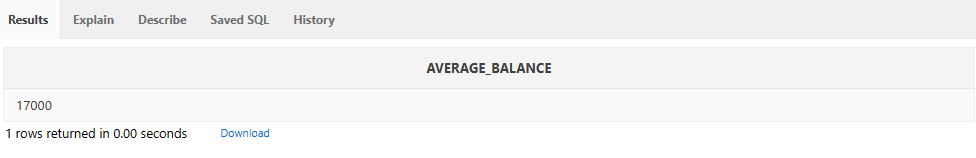
\includegraphics[width=0.9\textwidth]{images/dml/GroupFun/Q1.png}
    \caption{Result of Query 1}
    \label{fig:Result of Query 1}
\end{figure}
%%%
\begin{itemize}
    \item Count the number of teams established in each country
\end{itemize}

\begin{lstlisting}[caption={ Query 2},label={lst:q-2}]
    SELECT Team_Country, COUNT(*) AS Team_Count
    FROM Team
    GROUP BY Team_Country;
\end{lstlisting}

\begin{figure}[H]
    \centering
    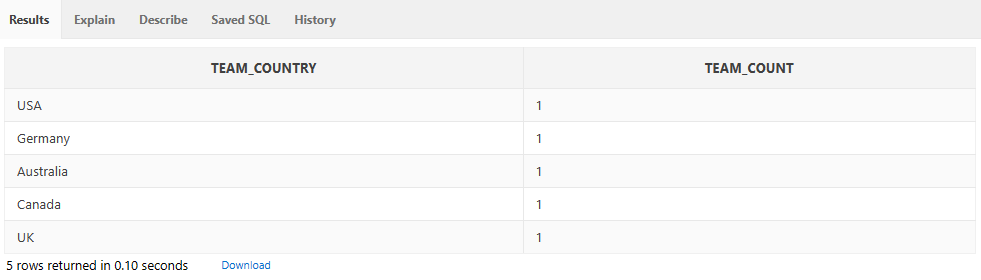
\includegraphics[width=0.9\textwidth]{images/dml/GroupFun/Q2.png}
    \caption{Result of Query 2}
    \label{fig:Result of Query 2}
\end{figure}
%%%

\begin{itemize}
    \item Calculate the total salary expense for content creators
\end{itemize}

\begin{lstlisting}[caption={ Query 3},label={lst:q-3}]
    SELECT SUM(ContentCreator_Salary) AS Total_Salary_Expense
    FROM ContentCreator;
\end{lstlisting}
\begin{figure}[H]
    \centering
    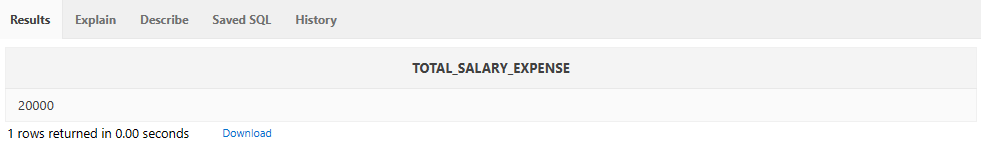
\includegraphics[width=0.9\textwidth]{images/dml/GroupFun/Q3.png}
    \caption{Result of Query 3}
    \label{fig:Result of Query 3}
\end{figure}
\clearpage